% !TEX TS-program = pdflatex
% !TEX encoding = UTF-8 Unicode

% This is a simple template for a LaTeX document using the "article" class.
% See "book", "report", "letter" for other types of document.

\documentclass[11pt]{article} % use larger type; default would be 10pt

\usepackage[utf8]{inputenc} % set input encoding (not needed with XeLaTeX)

%%% Examples of Article customizations
% These packages are optional, depending whether you want the features they provide.
% See the LaTeX Companion or other references for full information.

%%% PAGE DIMENSIONS
\usepackage{geometry} % to change the page dimensions
\geometry{a4paper} % or letterpaper (US) or a5paper or....
\geometry{margin=0.5in} % for example, change the margins to 2 inches all round
% \geometry{landscape} % set up the page for landscape
%   read geometry.pdf for detailed page layout information

\usepackage{graphicx} % support the \includegraphics command and options

% \usepackage[parfill]{parskip} % Activate to begin paragraphs with an empty line rather than an indent

%%% PACKAGES
\usepackage{booktabs} % for much better looking tables
\usepackage{array} % for better arrays (eg matrices) in maths
\usepackage{paralist} % very flexible & customisable lists (eg. enumerate/itemize, etc.)
\usepackage{verbatim} % adds environment for commenting out blocks of text & for better verbatim
\usepackage{subfig} % make it possible to include more than one captioned figure/table in a single float
% These packages are all incorporated in the memoir class to one degree or another...

%%% HEADERS & FOOTERS
\usepackage{fancyhdr} % This should be set AFTER setting up the page geometry
\pagestyle{fancy} % options: empty , plain , fancy
\renewcommand{\headrulewidth}{0pt} % customise the layout...
\lhead{}\chead{}\rhead{}
\lfoot{}\cfoot{\thepage}\rfoot{}

%%% SECTION TITLE APPEARANCE
\usepackage{sectsty}
\allsectionsfont{\sffamily\mdseries\upshape} % (See the fntguide.pdf for font help)
% (This matches ConTeXt defaults)

%%% ToC (table of contents) APPEARANCE
\usepackage[nottoc,notlof,notlot]{tocbibind} % Put the bibliography in the ToC
\usepackage[titles,subfigure]{tocloft} % Alter the style of the Table of Contents
\renewcommand{\cftsecfont}{\rmfamily\mdseries\upshape}
\renewcommand{\cftsecpagefont}{\rmfamily\mdseries\upshape} % No bold!

%%% END Article customizations

%%% The "real" document content comes below...

\title{Week 3 Assignment}
\author{Efeosa Eguavoen - 17324649}
%\date{} % Activate to display a given date or no date (if empty),
         % otherwise the current date is printed 

\begin{document}
\maketitle

\section{(i) - id:2--2-2}
\subsection{a}
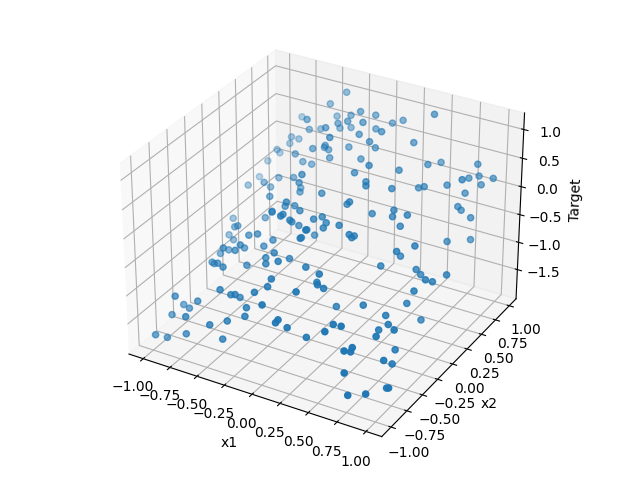
\includegraphics[scale=0.5]{3Ddata.jpg}
\\
To generate the graph, I first read in the data and placed it into a dataframe. I then used ax.scatter to generate the 3d graph and added labels using built in functions to label my axes. 
\begin{verbatim}
fig = plt.figure()
ax = fig.add_subplot(111, projection='3d')
ax.scatter(df['x1'], df['x2'], df['label'])
ax.set_xlabel('x1')
ax.set_ylabel('x2')
ax.set_zlabel('Target')
\end{verbatim}
The graph seems to have some sort of curve shape, as the data points towards the front of the graph go up in the centre then down, indicating some sort of quadratic shape roughly. 

\subsection{b}
Below is a list of parameters and their values, assigned by the feature the parameter represents i.e parameter  \(x1\) would represent the feature x1 in our model.
\\\\
C = 1e-07, \(\theta_0\)= 0.0445 , \(x1\)= -0.07552 ,\(x2\)= 1.14206 , \(x1^2\)= -1.22412 , \(x1 x2\)= -0.02332 , \(x2^2\)= 0.05937 , \(x1^3\)= -0.05101, \(x1^2 x2\)= -0.27161 , \(x1 x2^2\)= 0.13406 , \(x2^3\)= -0.41954 , \(x1^4\)= 0.13894 , \(x1^3 x2\) 0.18631 , \(x1^2 x2^2\)= 0.23999 , \(x1 x2^3\)= -0.10213 , \(x2^4\)= -0.157 , \(x1^5\)= 0.23727 , \(x1^4 x2\)= 0.21418 , \(x1^3 x2^2\)= -0.45974 , \(x1^2 x2^3\)= 0.11804 , \(x1 x2^4\)= 0.16536 , \(x2^5\)=0 \\\\
 C = 0.0001, \(\theta_0\)= 0.04026 , \(x1\)= -0.06351 ,\(x2\)= 1.06087 , \(x1^2\)= -1.17545 , \(x1 x2\)= -0.02465 , \(x2^2\)= 0.04517 , \(x1^3\)= -0.0, \(x1^2 x2\)= -0.07107 , \(x1 x2^2\)= 0.01734 , \(x2^3\)= -0.18706 , \(x1^4\)= 0.09282 , \(x1^3 x2\) 0.17555 , \(x1^2 x2^2\)= 0.21429 , \(x1 x2^3\)= -0.08526 , \(x2^4\)= -0.13633 , \(x1^5\)= 0.14509 , \(x1^4 x2\)= 0.0583 , \(x1^3 x2^2\)= -0.31226 , \(x1^2 x2^3\)= 0.00144 , \(x1 x2^4\)= 0.20766 , \(x2^5\)=0 \\\\
 C = 0.001, \(\theta_0\)= 0.02515 , \(x1\)= -0.01396 ,\(x2\)= 1.00104 , \(x1^2\)= -1.03751 , \(x1 x2\)= -0.0 , \(x2^2\)= -0.0 , \(x1^3\)= 0.0, \(x1^2 x2\)= -0.0 , \(x1 x2^2\)= 0.0 , \(x2^3\)= 0.0 , \(x1^4\)= -0.0 , \(x1^3 x2\) 0.06204 , \(x1^2 x2^2\)= 0.06914 , \(x1 x2^3\)= -0.00465 , \(x2^4\)= -0.0316 , \(x1^5\)= 0.0 , \(x1^4 x2\)= -0.0 , \(x1^3 x2^2\)= -0.0 , \(x1^2 x2^3\)= -0.0 , \(x1 x2^4\)= 0.00195 , \(x2^5\)=0 \\\\
 C = 0.01, \(\theta_0\)= -0.01231 , \(x1\)= -0.0 ,\(x2\)= 0.97702 , \(x1^2\)= -0.91498 , \(x1 x2\)= 0.0 , \(x2^2\)= -0.0 , \(x1^3\)= -0.0, \(x1^2 x2\)= 0.0 , \(x1 x2^2\)= -0.0 , \(x2^3\)= 0.0 , \(x1^4\)= -0.0 , \(x1^3 x2\) 0.0 , \(x1^2 x2^2\)= -0.0 , \(x1 x2^3\)= 0.0 , \(x2^4\)= -0.0 , \(x1^5\)= -0.0 , \(x1^4 x2\)= 0.0 , \(x1^3 x2^2\)= -0.0 , \(x1^2 x2^3\)= 0.0 , \(x1 x2^4\)= -0.0 , \(x2^5\)=0 \\\\
 C = 0.1, \(\theta_0\)= -0.31178 , \(x1\)= -0.0 ,\(x2\)= 0.72438 , \(x1^2\)= -0.0 , \(x1 x2\)= -0.0 , \(x2^2\)= -0.0 , \(x1^3\)= -0.0, \(x1^2 x2\)= 0.0 , \(x1 x2^2\)= -0.0 , \(x2^3\)= 0.0 , \(x1^4\)= -0.0 , \(x1^3 x2\) 0.0 , \(x1^2 x2^2\)= -0.0 , \(x1 x2^3\)= -0.0 , \(x2^4\)= -0.0 , \(x1^5\)= -0.0 , \(x1^4 x2\)= 0.0 , \(x1^3 x2^2\)= -0.0 , \(x1^2 x2^3\)= 0.0 , \(x1 x2^4\)= -0.0 , \(x2^5\)=0 \\\\
 C = 1, \(\theta_0\)= -0.31477 , \(x1\)= -0.0 ,\(x2\)= 0.0 , \(x1^2\)= -0.0 , \(x1 x2\)= -0.0 , \(x2^2\)= -0.0 , \(x1^3\)= -0.0, \(x1^2 x2\)= 0.0 , \(x1 x2^2\)= 0.0 , \(x2^3\)= 0.0 , \(x1^4\)= -0.0 , \(x1^3 x2\) 0.0 , \(x1^2 x2^2\)= -0.0 , \(x1 x2^3\)= -0.0 , \(x2^4\)= -0.0 , \(x1^5\)= 0.0 , \(x1^4 x2\)= 0.0 , \(x1^3 x2^2\)= 0.0 , \(x1^2 x2^3\)= 0.0 , \(x1 x2^4\)= 0.0 , \(x2^5\)=0 \\\\


As the value of C changes, more and more of my parameters reduce in size and eventually become 0. This is due to the L1 penalty which sets parameters to 0 to remove the less important features.
\\To get the features, I used PolynomialFeatures fitted to the data given to us, to the power of 5. I then placed this into a dataframe called features, with each feature labelled accordingly like in the photo below.
\begin{verbatim}
 p = PolynomialFeatures(5).fit(df[['x1', 'x2']])
    features = pd.DataFrame(p.transform(df[['x1', 'x2']]), columns=p.get_feature_names(df.columns))
\end{verbatim}
After this I then had a list of C vals between 0 and 1 as 1 was where I found my parameter values to all equal 0, so I used a range of values between 0 and 1 as my C values. From there I used a for loop to iterate through my values of C and created a model for each value of C, fitting the data and added each model to my list of models. 
\begin{verbatim}
models = []
    c_vals = [1e-7, 1e-4, 1e-3, 1e-2, 1e-1, 1]
    for s in c_vals:
        model = Lasso(alpha=s)
        model.fit(features, df['label'])
        models.append((model, s))
\end{verbatim}
\subsection{C}
\begin{figure}[h]
\centering
\subfloat[C = 1e-07]{{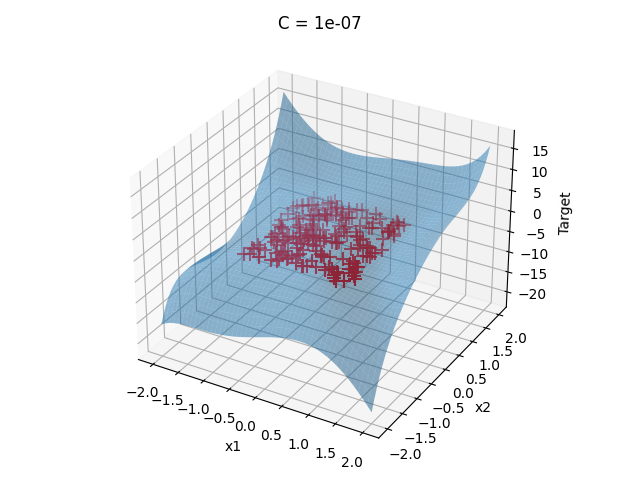
\includegraphics[width=5cm]{p1.jpg}}}
\qquad
\subfloat[C = 0.0001]{{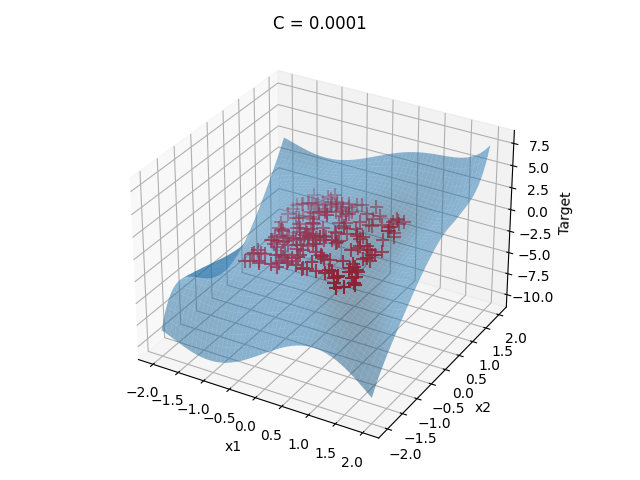
\includegraphics[width=5cm]{p2.jpg}}}
\qquad
\subfloat[C = 0.001]{{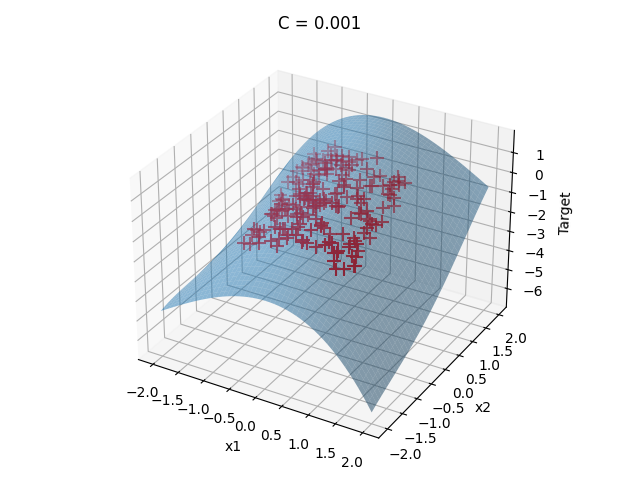
\includegraphics[width=5cm]{p3.jpg}}}
\qquad
\subfloat[C = .01]{{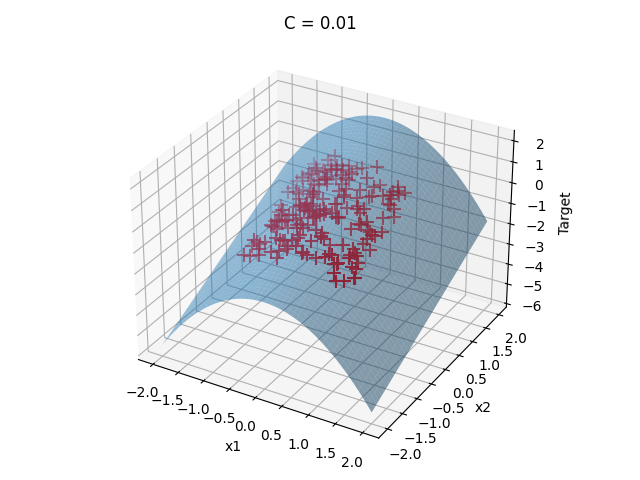
\includegraphics[width=5cm]{p4.jpg}}}
\qquad
\subfloat[C = .1]{{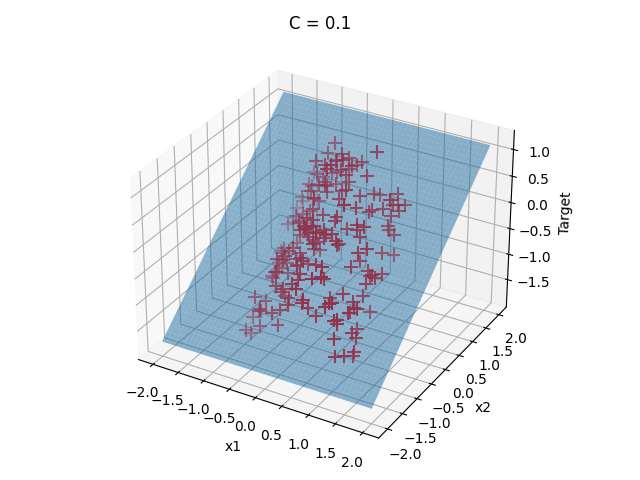
\includegraphics[width=5cm]{p5.jpg}}}
\qquad
\subfloat[C = 1]{{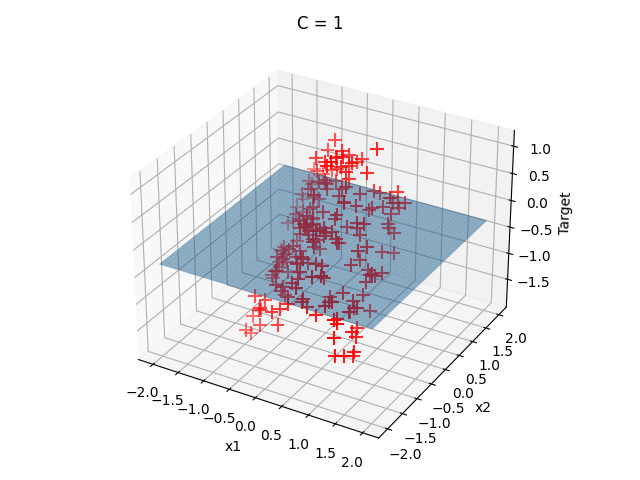
\includegraphics[width=5cm]{p6.jpg}}}
\end{figure}
 Red Dots: Training Data, Blue curves: Predictions (Adding a legend to a 3d plot isn't natively supported).\\
 From the above plots we can see that changing the value of C influences hugely our predictions. This is due to the fact that Lasso regression uses a L1 penalty that sets more and more of our parameters to 0 as we increase the value of C. This can be seen as the shapes of our graph change a lot, for example when C = 1e-07 the shape of the predictions is quite wild and fits the data closely, while when C = 1 it doesn't fit the data at all, as all our parameters are set to 0.
 \\
 To generate these graphs, I created a list of points for x1 and x2, then I used np.meshgrid to generate a grid of points. From there I flattened the arrays to 1D and stacked them using np.ravel and np.vstack respectively. I got the transpose of this array which then acted as my base array to generate features from using Polynomial features.
 \begin{verbatim}
x1vals = y1vals = np.array(np.linspace(-2, 2))
x, y = np.meshgrid(x1vals, y1vals)
positions = np.vstack([x.ravel(), y.ravel()])
xtest = (np.array(positions)).T
pdata = pd.DataFrame(xtest, columns=['x1', 'x2'])
p1 = PolynomialFeatures(5).fit(pdata[['x1', 'x2']])
mesh_features = pd.DataFrame(p1.transform(pdata[['x1', 'x2']]), columns=p.get_feature_names(pdata.columns))
 \end{verbatim}
 From here I iterated over my list of models and made predictions on the dataframe of data points and plotted each graph of predictions vs the training data.
 \begin{verbatim}
     for i in models:
        pred = i[0].predict(mesh_features)
        pred = pred.reshape(x.shape)
 \end{verbatim}
 \subsection{D}
 Overfitting refers to a model that matches the training data too closely, to the point where it's capturing all the noise and randomness in the graph. Underfitting refers to a model that doesn't capture the trends of the data at all and can't make accurate predictions of the data whatsoever. The parameter C enables us to manage between overfitting and underfitting our data by setting more of our parameter values to 0 in terms of Lasso Regression. This enables us to ignore certain parameters that aren't as important in capturing the general trend in the data. We can see this in the graph where C = 0.001 compared to when C = 0.0001. More of our parameters have been set to 0 or values very close to 0, which in turn enables us to capture the general shape of the data without overfitting like when C = 0.0001. When this penalty is too aggressive though we can get an underfit, like when C = .1 vs C = 0.01
 \subsection{E}
C = 0.1, P1= 0.03095 , P2 -0.05826, P3 = 1.0492 ,P4= -1.11603 , P5= -0.03996 , P6= 0.06502 , P7= -0.03677 , P8= -0.09889, P9= 0.04799 , P10= -0.14877 , P11= 0.03617 , P12= 0.19125 , P13 0.19494 , P14=0 -0.0765 , P15= -0.15176 , P16 0.17512 , P17= 0.087 , P18= -0.31386 , P19= 0.01242 , P20= 0.17554 , P21 0.12151\\\\ 
 C = 1, P1= -0.01188 , P2 -0.03962, P3 = 0.92238 ,P4= -0.78047 , P5= -0.03828 , P6= 0.04725 , P7= 0.00321 , P8= 0.05269, P9= 0.00714 , P10= 0.11186 , P11= -0.25642 , P12= 0.14868 , P13 0.05151 , P14=0 -0.03095 , P15= -0.08272 , P16 0.05163 , P17= -0.0039 , P18= -0.10055 , P19= -0.07439 , P20= 0.07778 , P21 -0.00955\\\\ 
 C = 10, P1= -0.08996 , P2 -0.02814, P3 = 0.66836 ,P4= -0.45295 , P5= -0.00747 , P6= 0.02016 , P7= -0.00154 , P8= 0.10677, P9= -0.01041 , P10= 0.23672 , P11= -0.33156 , P12= 0.04811 , P13 -0.09265 , P14=0 -0.01277 , P15= -0.00856 , P16 0.00461 , P17= 0.03698 , P18= -0.01775 , P19= 0.01199 , P20= 0.00332 , P21 0.10503\\\\ 
 C = 100, P1= -0.23009 , P2 -0.02313, P3 = 0.31862 ,P4= -0.14083 , P5= -0.00641 , P6= -0.0079 , P7= -0.00516 , P8= 0.09755, P9= -0.00469 , P10= 0.18004 , P11= -0.11592 , P12= 0.00663 , P13 -0.0489 , P14=0 -0.00815 , P15= -0.01303 , P16 -0.00051 , P17= 0.05749 , P18= 0.00114 , P19= 0.05736 , P20= 0.00156 , P21 0.12409 \\\\
 C = 1000, P1= -0.30216 , P2 -0.00362, P3 = 0.06161 ,P4= -0.01868 , P5= -0.00123 , P6= -0.00256 , P7= -0.00052 , P8= 0.0213, P9= 5e-05 , P10= 0.03766 , P11= -0.01556 , P12= 0.00086 , P13 -0.00742 , P14=0 -0.00135 , P15= -0.00332 , P16 0.00028 , P17= 0.01324 , P18= 0.00108 , P19= 0.01357 , P20= 0.0011 , P21 0.02723\\\\ 
 C = 10000, P1= -0.31343 , P2 -0.00037, P3 = 0.00683 ,P4= -0.00194 , P5= -0.00013 , P6= -0.00029 , P7= -4e-05 , P8= 0.00239, P9= 3e-05 , P10= 0.00421 , P11= -0.00161 , P12= 9e-05 , P13 -0.00079 , P14=0 -0.00014 , P15= -0.00038 , P16 5e-05 , P17= 0.0015 , P18= 0.00014 , P19= 0.00154 , P20= 0.00014 , P21 0.00306\\\\ 

 \begin{figure}[h]
\centering
\subfloat[C = 0.1]{{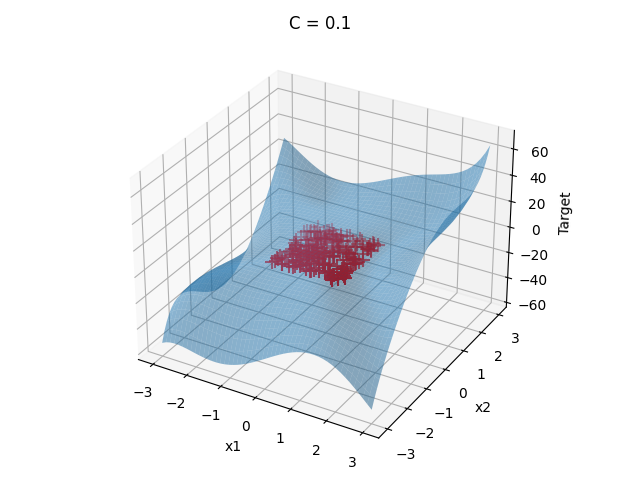
\includegraphics[width=5cm]{r1.jpg}}}
\qquad
\subfloat[C = 1]{{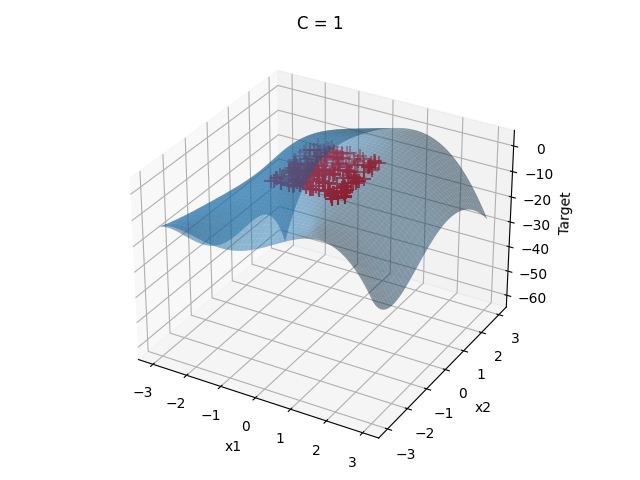
\includegraphics[width=5cm]{r2.jpg}}}
\qquad
\subfloat[C = 10]{{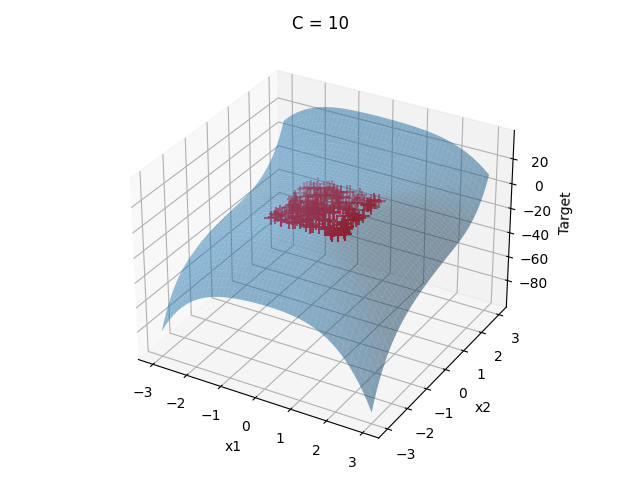
\includegraphics[width=5cm]{r3.jpg}}}
\qquad
\subfloat[C = 100]{{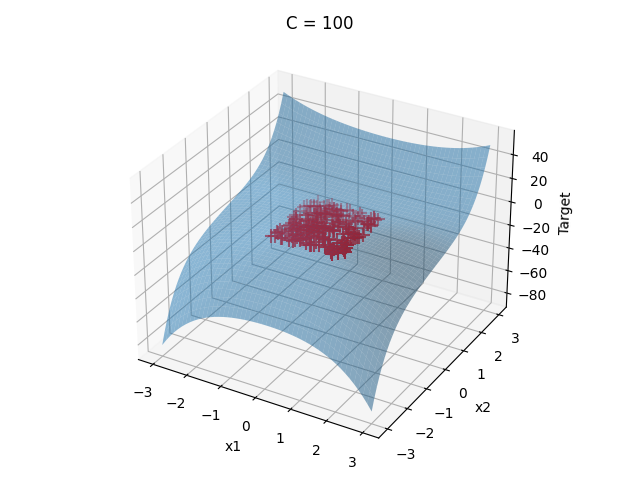
\includegraphics[width=5cm]{r4.jpg}}}
\qquad
\subfloat[C = 1000]{{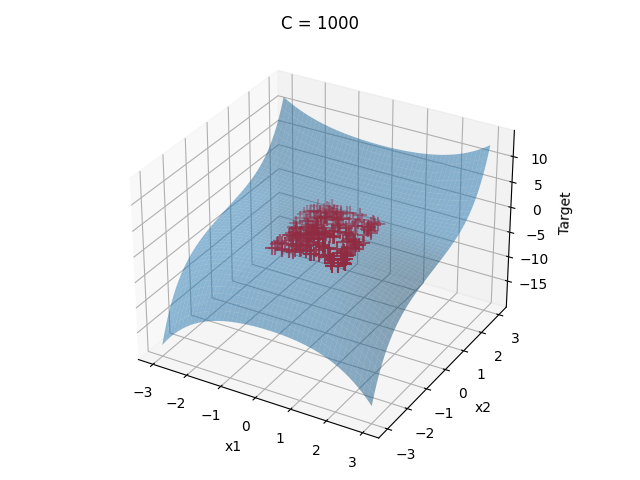
\includegraphics[width=5cm]{r5.jpg}}}
\qquad
\subfloat[C = 10,000]{{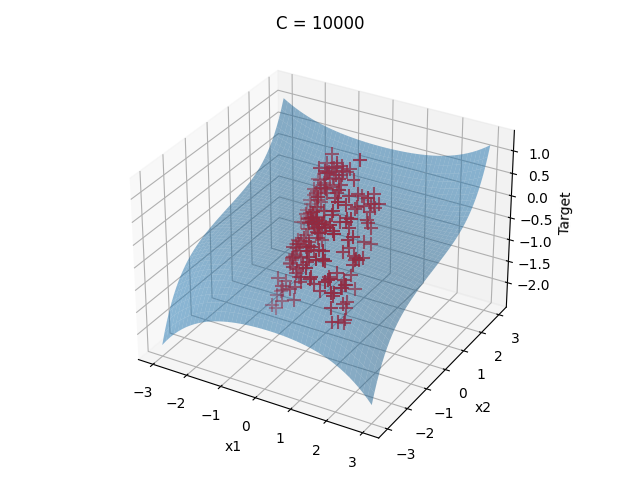
\includegraphics[width=5cm]{r6.jpg}}}
\end{figure}
From the graphs below, we can see that when using Ridge Regression, our value of C behaves rather differently to Lasso Regression. For small values of C i.e in graph(a), it overfits the data. But in Lasso regression, for a similar C value, the model doesn't overfit the data at all. The L2 Penalty used in Ridge Regression doesn't set any of our parameters to 0, rather it reduces the weight of that parameter to a value approaching 0 as the magnitude of the penalty increases. We can see this in graph (f) where C = 10,000 where we get a underfit of the data. Our parameter values above also are all very small, with values approaching 0. It seems Ridge Regression works well to prevent overfitting the data unless we use very small values of C, while Lasso Regression helps us with feature selection as it can discount features that aren't important by setting their parameters to 0.
\section{(ii)} 
\subsection{A}
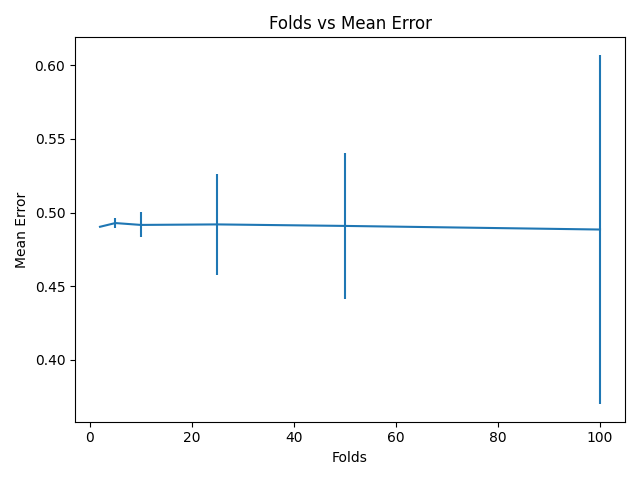
\includegraphics[scale=0.4]{fold.jpg}
\\
When selecting the number of folds, there's a trade off between the amount of computational time we can use and the level of bias we're willing to accept. Having higher values of K enables us to have less bias overall as the training set better represents the data and the variance increases as the training sets become more similar. But having too high a value of K becomes an issue as the test set might become too small which might not properly represent the data. For this dataset, I think using a value of K = 10 is appropriate as the data set isn't that large and using larger values of K reduces or test set too much to represent the data well. Using 5 increases the mean error slightly also.
\\ To get the above graph, I set up a list of K values and a list for mean errors and their associated variances.  I then iterated over this list of K values to generate different splits.
\begin{verbatim}
k_vals = [2, 5, 10, 25, 50, 100]
mean_list = []
variance_list = []
    for k in k_vals:
        error_list = []
        kf = KFold(n_splits=k)
\end{verbatim}
I then split the training data into 2 sets, a training set and a test set. Following this I trained the model and got the mean squared error and appended this to the error list. Once I had all the errors, I got the mean and variance and appended them to their respective lists. I then plotted after.
 \begin{verbatim}
         for train, test in kf.split(features):
            x_train, x_test = features.loc[train], features.loc[test]
            y_train, y_test = df.loc[train, 'label'], df.loc[test, 'label']
            model = Lasso(alpha=1)
            model.fit(x_train.values, y_train.values)
            pred = model.predict(x_test)
            error_list.append(mean_squared_error(y_test.values, pred))
        error_list = np.array(error_list)
        mean = error_list.mean()
        mean_list.append(mean)
        var = error_list.var()
        variance_list.append(var)
 \end{verbatim}
\subsection{B}
\begin{figure}[h]
\subfloat[0 \(<\) C \(<\) 1]{{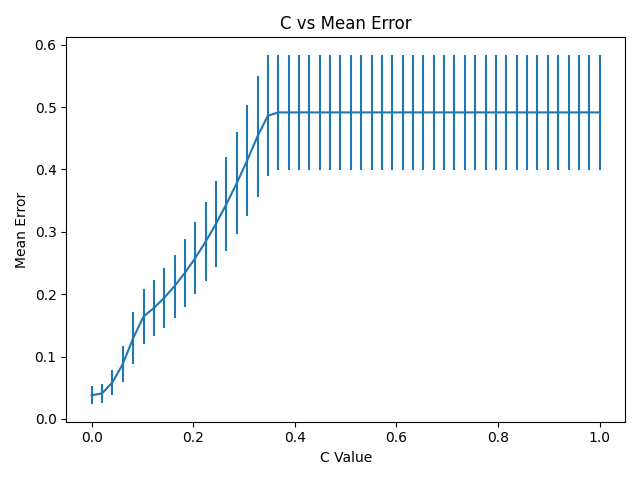
\includegraphics[width=8cm]{c1.jpg}}}
\qquad
\subfloat[0 \(<\) C \(<\) 0.1]{{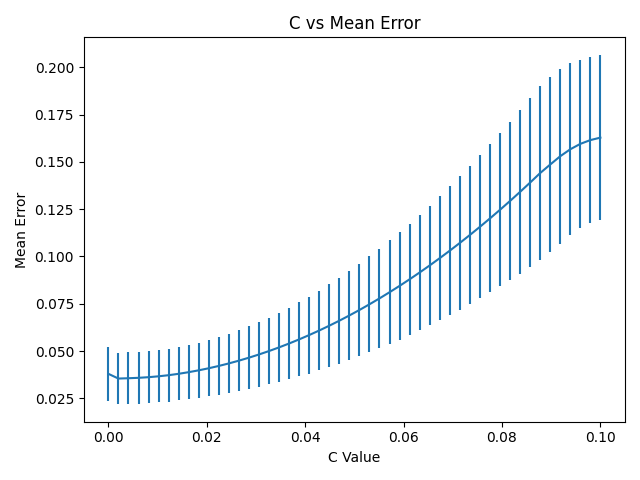
\includegraphics[width=8cm]{c2.jpg}}}
\end{figure}
I used 10-fold Cross validation for the above plots as I established it to work slightly better than 5 fold in an earlier section. For choosing values of C, I first started with mapping values between 0 and 1 like in the plot(a) as this spanned all values of C that kept my parameters non 0. From there I then reduced the range to scan values of C as I could see that towards the left of graph(a) was where my minimum was. From there I generated graph(b) which scans values in a much smaller range to find the optimum value of C.
\\
To generate the graphs, I used the same code as for using different values of K, I just iterated over my list of C values instead of iterating through a list of values of K.
\begin{verbatim}
c_vals = np.linspace(0.00000001, 0.1)
    mean_list = []
    std_list = []
    kf = KFold(n_splits=10)
    for i in c_vals:
\end{verbatim}

\subsection{C}
Based on the above graph, I'd recommend a value of C around 0.002 as the values of C seem to take a slight dip at the start around C = 0.02 then just increases from there. At this point, my mean square error is at it's lowest meaning the accuracy of my predictions is at it's best here as the parameters of my algorithm are the most optimised they can be and are as accurate to the trends in the data as possible.
\subsection{D}
\begin{figure}[h]
\subfloat[0 \(<\) C \(<\) 1]{{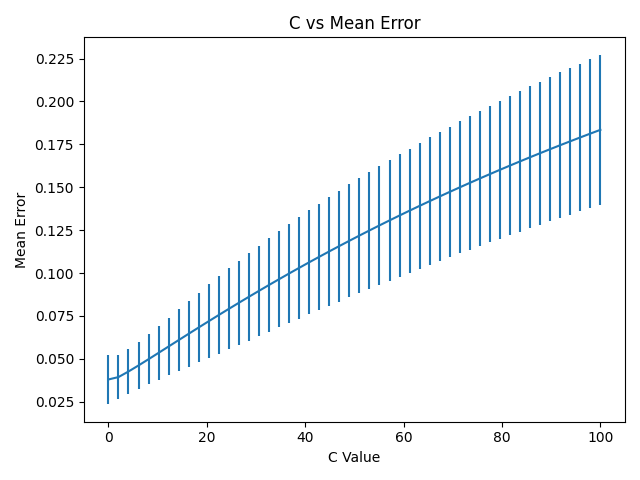
\includegraphics[width=8cm]{rc1.jpg}}}
\qquad
\subfloat[0 \(<\) C \(<\) 0.1]{{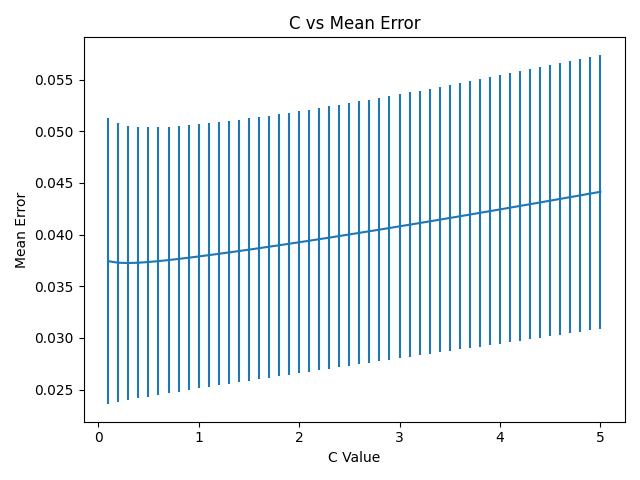
\includegraphics[width=8cm]{rc2.jpg}}}
\end{figure}
To choose a range for C, I started with a larger range of values, beween 0 and 100, then I zoomed in on the lower end of the range where my C values seem to dip, between 0 and 5.\\\\ I'd recommend using a value of around C = 0.5 for Ridge regression as at that point on graph(b) is the lowest point where the mean error is lowest. 
\end{document}
